\section{Sprint Report}

\subsection{Current Sprint}

The following stories was completed as planed at the start of the sprint:
\begin{itemize}
    \item Create code that can connect to LinkedIn.
    \item Create a (simple, non-intergrated) login portal to let the user provide their linkedin credentials/API-key. 
    \item Create code that can extract information from LinkedIn.
    \item Create code that can translate extracted LinkedIn information into Leapkit information.
    \item Research matching methods for the algorithm.
\end{itemize}
We did not complete the story:
\begin{center}
    Create code that can save the translated LinkedIn data to the Leapkit Database.
\end{center}
As we in the sprint discovered we needed more information about the database from our product owner. The slowdown seen on our burndown chart (Figure \ref{fig:burndownSprint}) is explained by us running into the problem of installing and running the virtual machine that is needed for us to code on the project.\\
\begin{figure}[!ht]
    \centering
    \begin{subfigure}[b]{0.5\textwidth}
        \scalebox{.6}{\begin{tikzpicture}

% horizontal axis
    \draw[->] (0,0) -- (8,0) node[anchor=north] {\emph{Day}};
% labels
    \draw   (0,0) node[anchor=north] {0}
            (1,0) node[anchor=north] {1}
            (2,0) node[anchor=north] {2}
            (3,0) node[anchor=north] {3}
            (4,0) node[anchor=north] {4}
            (5,0) node[anchor=north] {5}
            (6,0) node[anchor=north] {6}
            (7,0) node[anchor=north] {7};

% vertical axis
    \draw[->] (0,0) -- (0,8) node[anchor=east] {\emph{Points remaining}};
% labels
    \draw   (0,1) node[anchor=east] {3}
            (0,2) node[anchor=east] {5.5}
            (0,3) node[anchor=east] {8}
            (0,4) node[anchor=east] {10.5}
            (0,5) node[anchor=east] {12}
            (0,6) node[anchor=east] {15.5}
            (0,7) node[anchor=east] {18};

% projected 
    \draw[thick, dotted, red] (0,7) -- (7,0);

% actual
    \draw[thick, blue] (0,7) -- (1,6.5) -- (2,6.0) -- (3,4) -- (4,2.5) -- (5,2.5) -- (6,1); 
   
% legend
    \begin{scope}[shift={(4,4)}] 
        \draw[thick, dotted, red] (0,0) -- (0.5,0) 
            node[black, right]{Projected Sprint};
        \draw[thick, blue, yshift=\baselineskip] (0,0) -- 
            plot[] (0.25,0) -- (0.5,0)
            node[black, right]{Actual Sprint};
    \end{scope}
\end{tikzpicture}
}
        \caption{Burndown of the current sprint}
        \label{fig:burndownSprint}
    \end{subfigure}%
    \begin{subfigure}[b]{0.5\textwidth}
        \scalebox{.7}{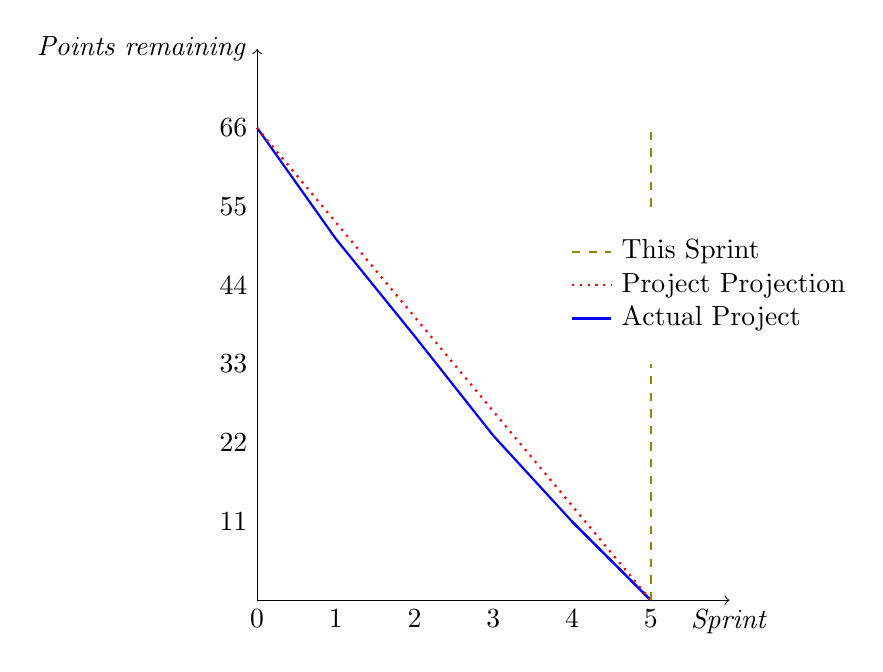
\begin{tikzpicture}

% horizontal axis
    \draw[->] (0,0) -- (6,0) node[anchor=north] {\emph{Sprint}};
% labels
    \draw   (0,0) node[anchor=north] {0}
            (1,0) node[anchor=north] {1}
            (2,0) node[anchor=north] {2}
            (3,0) node[anchor=north] {3}
            (4,0) node[anchor=north] {4}
            (5,0) node[anchor=north] {5};

% vertical axis
    \draw[->] (0,0) -- (0,7) node[anchor=east] {\emph{Points remaining}};
% labels
    \draw   (0,1) node[anchor=east] {11}
            (0,2) node[anchor=east] {22}
            (0,3) node[anchor=east] {33}
            (0,4) node[anchor=east] {44}
            (0,5) node[anchor=east] {55}
            (0,6) node[anchor=east] {66};
% actual
    \draw[thick, blue] (0,6) -- (1,4.59) -- (2,3.355) -- (3,2.09)-- (4,1.00) -- (5,0);
% actual projected
    \draw[thick, dashed, blue] (4,1.00) -- (5,0);

% projected 
    \draw[thick, dotted, red] (0,6) -- (5,0);


% current sprint 
    \draw[thick, dashed, olive] (5,0) -- (5,3);
    \draw[thick, dashed, olive] (5,5) -- (5,6);


    
\begin{scope}[shift={(4,4)}] 
    \draw[thick, dotted, red] (0,0) -- (0.5,0) 
        node[black, right]{Project Projection};
    \draw[thick, blue, yshift=\baselineskip * - 1] (0,0) -- (0.5,0)
        node[black, right]{Actual Project};
    \draw[thick, dashed, olive, yshift=\baselineskip] (0,0) -- (0.5,0)
        node[black, right]{This Sprint};
\end{scope}

\end{tikzpicture}
}
        \caption{Burndown of the project}
        \label{fig:burndownProject}
    \end{subfigure}
    \caption{Burndown charts}
\end{figure}
A general overview of the project can be seen on the general burndown chart (Figure \ref{fig:burndownProject}).\\
Observe that even though we did not complete everything we planed in the sprint, we did end up completing a larger amount of points than we projected, as multiple new stories were discovered and solved while we were working on the sprint. These include:
\begin{itemize}
    \item Setup virtual enviroment 
    \item Setup version control
    \item Setup continuous integration
\end{itemize}

\subsection{Next Sprint}

\begin{itemize}
    \item Create code that can save the translated LinkedIn data to the Leapkit Database.
    \item Setup Jenkins environment
    \item Implement basic match making algorithm ready for iterative developement/extensions
    \item Create test suite for the code generated in the previous sprint.
\end{itemize}

% stories completed, progress report (e.g., through a burndown chart), next sprint
